\documentclass[]{article}

% accenti
\usepackage[utf8]{inputenc}
% rimuove indentatura
\usepackage[parfill]{parskip}
% colori
\usepackage{color}
% per cambiare i margini della pagina
\usepackage{vmargin}
% per fissare le figure
\usepackage{float}

\usepackage{graphicx}
\begin{document}

\title{Ricerca su sottoinsiemi individuati da N-grammi}
\author{Federico Magnolfi}
\date{Jun 4, 2017}
\maketitle


\section{Introduzione}
Si vuole analizzare l’utilità dell’utilizzo di N-grammi nella ricerca di parole in un lessico vicine ad una query (in termini di EditDistance).

\section{Descrizione}
\subsection*{EditDistance}
EditDistance è un algoritmo che misura la distanza tra due parole, essa è tanto più grande quanto più sono diverse le parole. Data una parola x, la distanza tra essa e una parola y è data dal minimo costo di operazioni elementari che permettono di trasformare la stringa x in y. Le operazioni elementari sono:
\begin{itemize}
\item copia di una lettera
\item inserimento di una lettera
\item modifica di una lettera
\item scambio tra due lettere
\item cancellazione di una lettera
\end{itemize}
Ad ogni operazione elementare corrisponde un costo che deve essere attribuito opportunamente.
In questo test si considera il costo di copia 0, il costo di ogni altra operazione 1.

\subsection*{Ricerca in un lessico}
Data una query Q, che non è altro che una parola, e un lessico L, ovvero un insieme di parole, è interessante trovare la distanza minima tra Q ed ogni altra parola di L.
Se Q appartiene ad L, la distanza minima sarà ovviamente 0. Se così non fosse, potrebbe essere utile conoscere la parola del lessico più vicina a Q.
Questa idea viene ad esempio utilizzata quando si commette un errore nell'eseguire una query su un motore di ricerca.
Visto che in generale il lessico può essere esageratamente grande, i tempi di ricerca sarebbero molto inferiori se si riuscisse a ridurre l'insieme di ricerca a parole simili a Q.

\subsection*{N-Gram}
Data una stringa, i suoi n-grammi sono tutte le sue sottostringhe di lunghezza n.
Gli n-gram sono una possibile soluzione al ridurre il lessico L ad un insieme di parole simili a Q, essi possono essere sfruttati in vari modi.
Ad esempio, si può pensare di eseguire la ricerca nel sottoinsieme composto dalle parole che contengono almeno un n-gramma di Q.

\section{Analisi teorica}
L'insieme di parole può essere implementato nel calcolatore con varie strutture dati, ad esempio con una tavola hash. Questa struttura dati, se ben bilanciata, permette di trovare in tempo costante la chiave se presente.
Quindi ci si aspetta che la ricerca di parole appartenenti al lessico sia più veloce quando non si sfruttano gli n-grammi, in questo caso sarà predominante il tempo di creazione del sottoinsieme su cui cercare.

Nel caso in cui la parola non sia presente nel lessico, trovare quella più vicina significa guardare tutte le parole dell'insieme: in questo caso la ricerca che sfrutta gli n-grammi sarà sicuramente più rapida visto che l'insieme su cui viene fatta la ricerca è più piccolo del lessico L.

Visto che quando si sfruttano gli n-grammi la ricerca viene eseguita su un sottoinsieme di L, esiste la possibilità che la ricerca produca un risultato differente rispetto alla ricerca su tutto L.

\section{Descrizione esperimenti}
Si usa come dizionario un file di testo contenente circa 660000 parole.
Si cercano alcune parole presenti nel dizionario e si misura il tempo di ricerca, analogamente si fa per parole non presenti.
La ricerca si effettua sul dizionario completo e sui sottoinsiemi creati con: 1-gram, 2-gram, 3-gram, 4-gram.
Le parole presenti cercate sono: "bacio", "come", "esame", "domanda", "veramente", "caratteristico".
Le parole non presenti cercate sono: "bscho", "cmoe", "seamee", "donamda", "versmenta", "carayyerisyico".

\subsection*{Piattaforma di test}
Il test viene eseguito su un computer desktop con le seguenti caratteristiche:
\begin{itemize}
\item Sistema Operativo: Linux Mint 18.1
\item CPU: Intel Core i5-2400 (6 MB cache, 3.40 Ghz)
\item RAM: 16 GB
\item linguaggio di programmazione e interprete: Python 3.5
\item IDE: PyCharm 2017
\end{itemize}

\section{Documentazione del codice}
Gli insiemi vengono implementati con i set, in modo da eseguire facilmente le unioni tra insiemi.
Il programma è composto da 3 file: edidistance.py,test.py, exp.py.

\subsection*{edidistance.py}
Implementa le funzioni utili al calcolo della distanza e degli n-grammi.
Le funzioni implementate sono le seguenti:
\begin{itemize}
\item editDistance(x, y): crea una matrice dove l'elemento i,j corrisponde alla distanza tra la sottostringa formata dai primi $i$ caratteri di x e tra la sottostringa formata dai primi $j$ caratteri di y.
\item distance(x, y): chiama la editDistance e restituisce il valore in fondo a destra della matrice, corrispondente alla distanza tra x e y
\item ngrams(string, n): restituisce una lista di tutti gli n-grammi di string
\end{itemize}

\subsection*{test.py}
Implementa le funzioni utili allo svolgimento dei test.
Contiene tre funzioni:
\begin{itemize}
\item findWord(parola, insieme): cerca la parola (stringa) nell'insieme (set); ritorna la distanza minima e la parola più vicina.
\item createDictionary(vocabolario, n): dato un vocabolario (set, corrispondente al lessico L), crea un dizionario avente n-grammi come chiavi e come valori l'insieme di parole contenenti l'n-gramma.
\item createSet(parola, dict, n): dato il dizionario creato in precedenza e la parola su cui si vuole fare la ricerca, ritorna l'unione degli insiemi corrispondenti a tutti gli n-grammi della parola.
\item test(vocabolario, parole, maxNGram): esegue la ricerca della lista delle parole nel dizionario, misurando i tempi di ricerca e facendone la media. Esegue questa operazione sia sul vocabolario completo, sia sfruttando i vari n-grammi fino al valore massimo indicato. Ritorna i risultati del test in due liste (tempi/distanze) i cui elementi sono formati nel seguente modo:
\begin{itemize}
\item tempi: [tempoInizializzazione, tempoMedioRicerca]
\item distanze: [distanzaPrimaParola, distanzaSecondaParola, ...]
\end{itemize}
\end{itemize}

\subsection*{exp.py}
A partire dal file $Dizionario.txt$, crea un set contenente tutte le parole del dizionario. Chiama successivamente la funzione di test, prima con la lista di parole presenti nel dizionario, poi con la lista di parole non presenti.

Analizza l'esito del test costruendo tre liste che saranno utili nella creazione degli istogrammi. Il formato di ogni lista è il seguente:
\begin{verbatim}
[dizCompleto, 1-gram, 2-gram, 3-gram, 4-gram]
\end{verbatim}

Le liste sono usate per creare tre istogrammi:
\begin{itemize}
\item il primo rappresenta i tempi di creazione dei dizionari che associano gli n-grammi agli insiemi di parole (Figura \ref{tempiInizializzazione}).
\item il secondo rappresenta i tempi medi di ricerca delle parole presenti (Figura \ref{tempiParolePresenti}).
\item il terzo rappresenta i tempi medi di ricerca delle parole non presenti (Figura \ref{tempiParoleNonPresenti}).
\end{itemize}

Per le distanze invece non verranno realizzati grafici.

\section{Risultati sperimentali}

I risultati ottenuti nella fase dei test sono i seguenti:
\begin{verbatim}
Parole presenti
  tempo: [[0, 0.0], [2.9781, 0.3649], [4.2679, 0.0902], [3.8295, 0.0149],
      [3.99, 0.002]]
  distanza: [[0, 0, 0, 0, 0, 0], [0, 0, 0, 0, 0, 0], [0, 0, 0, 0, 0, 0],
      [0, 0, 0, 0, 0, 0], [0, 0, 0, 0, 0, 0]]

Parole non presenti:
  tempo: [[0, 75.8932], [2.9156, 76.4908], [3.9117, 33.0663], [4.4086, 3.418],
      [3.8167, 0.5299]]
  distanza: [[2, 1, 2, 2, 2, 3], [2, 1, 2, 2, 2, 3], [2, 1, 2, 2, 2, 3],
      [2, 3, 2, 2, 2, 3], [5, 9223372036854775807, 2, 2, 2, 3]]
\end{verbatim}

Dopodiché vengono create le tre liste utili per la realizzazione degli istogrammi. Le liste sono le seguenti:

\begin{verbatim}
Tempi di inizializzazione:
    [0, 2.9781, 4.2679, 3.8295, 3.99]
    
Tempi medi di ricerca di parole presenti nel dizionario:
    [0.0, 0.3649, 0.0902, 0.0149, 0.002]
    
Tempi medi di ricerca di parole non presenti nel dizionario:
    [75.8932, 76.4908, 33.0663, 3.418, 0.5299]
\end{verbatim}

\begin{figure}[H]
	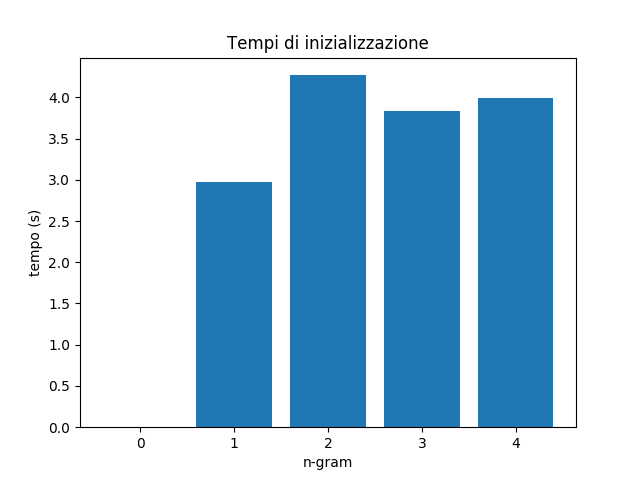
\includegraphics{tempi_inizializzazione.png}
	\caption{Tempi di creazione del sottoinsieme su sui fare la ricerca}
	\label{tempiInizializzazione}
\end{figure}

\begin{figure}[H]
	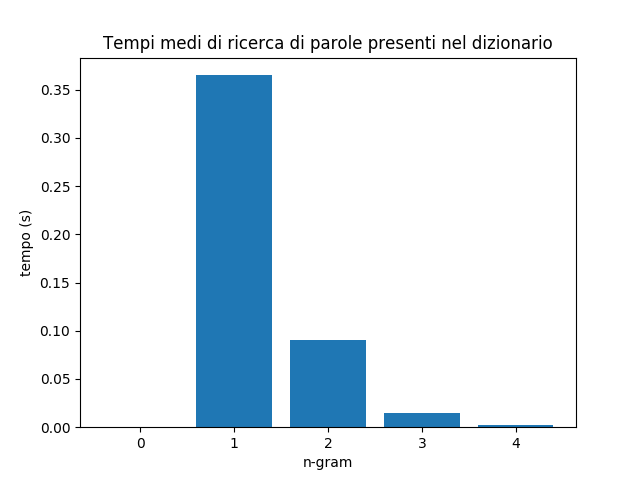
\includegraphics{tempi_ricerca_parole_presenti}
	\caption{Tempi medi di ricerca di parole presenti nel dizionario}
	\label{tempiParolePresenti}
\end{figure}

\begin{figure}[H]
	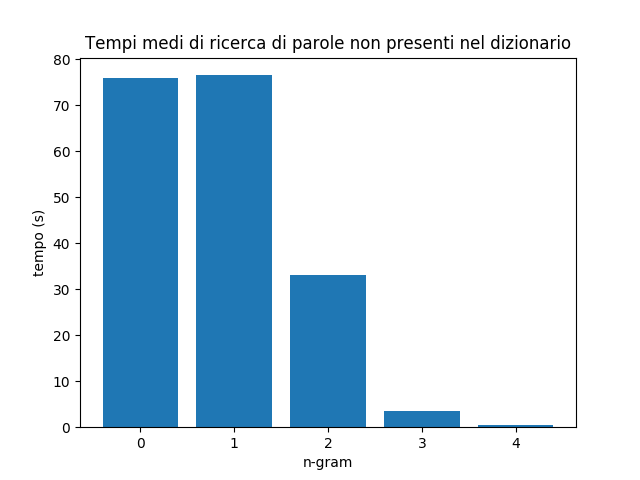
\includegraphics{tempi_ricerca_parole_non_presenti}
	\caption{Tempi medi di ricerca di parole non presenti nel dizionario}
	\label{tempiParoleNonPresenti}
\end{figure}


\section{Analisi dei risultati}
Il tempo di inizializzazione è ovviamente nullo per il dizionario completo, mentre per tutti gli n-grammi è molto simile.

Il tempo medio di ricerca di parole presenti nel vocabolario, è praticamente istantaneo nell'insieme completo coerentemente con le aspettative in quanto i set in python sono implementati con tabelle hash. Per gli n-grammi, il tempo misurato è il tempo di creazione del sottoinsieme su cui eseguire la ricerca: questi tempi, comunque piuttosto piccoli, decrescono al crescere di n.

I tempi medi di ricerca di parole non presenti nel vocabolario decresce il modo esponenziale all'aumentare di n. Esso è massimo quando la ricerca è effettuata sull'insieme completo oppure con il sottoinsieme fatto con gli 1-gram.

Quanto alle distanze minime, esse sono correttamente uguali a zero nel caso della ricerca di parole presenti.

Le distanze minime reali sono ovviamente quelle misurato nella ricerca sull'insieme totale: negli altri casi spesso rimangono corrette, tranne che per due parole:
\begin{itemize}
\item "bscho": simulazione di tasti premuti erroneamente (parola originale: "bacio"), la distanza minima è corretta fino ai 3-gram, è errata con i 4-gram.
\item "cmoe": simulazione di caratteri digitati in ordine errato (parola originale: "come"), la distanza minima è corretta fino ai 2-gram, è leggermente errata con i 3-gram; il numero che viene fuori nel caso dei 4-gram indica che la ricerca è stata effettuata su un insieme vuoto.
\end{itemize}
In entrambi i casi dove si sono verificate ricerche "errate" si nota che le parole erano molto brevi: il peso degli errori è maggiore del peso delle lettere corrette dopo un certo n-gramma.
Ricerche su insiemi vuoti si sarebbero verificate anche nel caso di ricerca di parole più brevi di n (esse non hanno n-grammi).

\section{Conclusioni}
Gli esiti dell'esperimento sono compatibili con ciò che era stato previsto.

Si ritiene quindi che per grossi insiemi di dati su cui trovare stringhe più simili, come ad esempio nel caso dei motori di ricerca, sia utile sfruttare i vantaggi dell'eseguire ricerche su sottoinsiemi più piccoli usando gli n-gram.

Si deve stare però attenti nel caso di parole brevi, in questo caso è preferibile eseguire ricerche su insiemi più ampi anche a discapito del tempo di esecuzione.

\end{document}